\documentclass[class=book, crop=false, oneside, 12pt]{standalone}
\usepackage{standalone}
\usepackage{amsmath}
\usepackage{../../style}
\graphicspath{{./assets/images/}}

\begin{document}

\chapter{Moti relativi}

\section{Sistemi di riferimento. Velocità e Accelerazione relative}

Sperimentalmente è provato con estrema accuratezza che le leggi fisiche non dipendono dalla scelta del sistema di riferimento. 
Fissato un sistema di riferimento e stabilita una certa proprietà, questa resta vera anche se cambiano l'origine e l'orientazione degli assi coordinati, ovvero se ci riferiamo ad un altro sistema ottenuto dal primo con una traslazione (spostamento dell'origine, conservando la stessa direzione degli assi) o con una rotazione (stessa origine, cambio della direzione degli assi) o con una operazione combinata.
Non esiste pertanto un punto privilegiato dello spazio e nemmeno un'orientazione privilegiata: lo spazio appare omogeneo e isotropo. 

\begin{figure}[h]
    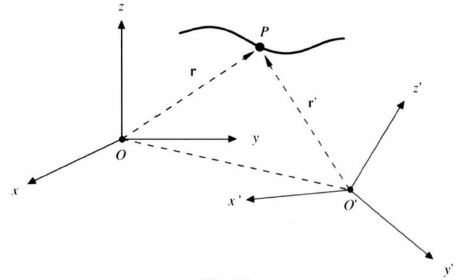
\includegraphics[scale=0.8]{punto_due_sistemi_riferimento}
    \centering
    \caption{}
    \label{punto_due_sistemi_riferimento}
\end{figure}

Abbiamo già rilevato come il concetto stesso di moto sia relativo,  abbia cioè bisogno della precisazione del sistema di riferimento. 
Consideriamo il problema riferendoci alla figura \ref{punto_due_sistemi_riferimento}. 
Il punto \(P\) è in movimento lungo una generica traiettoria. 
Il suo moto viene osservato da una terna cartesiana con centro in \(O\) che, per convenzione, chiamiamo sistema fisso e da una terna cartesiana con centro \(O'\) che, sempre per convenzione, chiamiamo sistema mobile.

Vogliamo ricavare una relazione tra la posizione, la velocità e l'accelerazione del punto \(P\), misurate da un osservatore solidale con il sistema fisso, e le corrispondenti grandezze misurate da un osservatore solidale con il sistema mobile. 

\subsection{Posizione}

La relazione tra le posizioni del punto \(P\), misurate rispetto ai due sistemi di riferimento, è la seguente:
\begin{equation} \label{pos_p}
    \overrightarrow{r} = \overrightarrow{OO'} + \overrightarrow{r'}
\end{equation}
con 
\begin{equation*}
    \overrightarrow{r} = x \overrightarrow{u_x} + y \overrightarrow{u_y} + z \overrightarrow{u_z} \ , \ \overrightarrow{r'} = x' \overrightarrow{u_{x'}} + y' \overrightarrow{u_{y'}} + z' \overrightarrow{u_{z'}} 
\end{equation*}
Assumiamo, dato che il primo sistema è fisso, che i versori \(\overrightarrow{u_x}, \overrightarrow{u_y}, \overrightarrow{u_z}\) sono indipendenti dal tempo.

\subsection{Velocità}

La velocità del punto \(P\) rispetto al sistema fisso, che chiamiamo velocità assoluta, è data da:
\begin{equation}
    \overrightarrow{v} = \frac{d \overrightarrow{r}}{dt} = \frac{dx}{dt} \overrightarrow{u_x} + \frac{dy}{dt} \overrightarrow{u_y} + \frac{dz}{dt} \overrightarrow{u_z}
\end{equation}
mentre quella misurata da un osservatore nel sistema mobile, che indichiamo come velocità relativa è
\begin{equation}
    \overrightarrow{v'} = \frac{dx'}{dt} \overrightarrow{u_{x'}} +\frac{dy'}{dt} \overrightarrow{u_{y'}} + \frac{dz'}{dt} \overrightarrow{u_{z'}}
\end{equation}
Infine la velocità dell origine \(O'\) del sistema di riferimento mobile misurata da un osservatore del sistema fisso e data da:
\begin{equation}
    \overrightarrow{v_{O'}}=\frac{d \overrightarrow{OO'}}{d t}=\frac{d x_{O'}}{d t} \overrightarrow{u_{x}}+\frac{d y_{O'}}{d t} \overrightarrow{u_{y}}+\frac{d z_{O'}}{d t} \overrightarrow{u_{z}}
\end{equation}

Derivando (\ref{pos_p}) rispetto al tempo ottengo

\begin{align*}
    \overrightarrow{v} = \frac{d \overrightarrow{r}}{dt} & = \frac{d \overrightarrow{OO'}}{d t} + \frac{d \overrightarrow{r'}}{dt} \\
    & = \frac{d x_{O'}}{d t} \overrightarrow{u_{x}}+\frac{d y_{O'}}{d t} \overrightarrow{u_{y}}+\frac{d z_{O'}}{d t} \overrightarrow{u_{z}}\\
        &+\frac{dx'}{dt} \overrightarrow{u_{x'}} + \frac{dy'}{dt} \overrightarrow{u_{y'}} + \frac{dz'}{dt} \overrightarrow{u_{z'}} + x' \frac{d\overrightarrow{u_{x'}}}{dt}  + y' \frac{d\overrightarrow{u_{y'}}}{dt}  + z' \frac{d\overrightarrow{u_{z'}}}{dt}\\
\end{align*}
ovvero
\begin{equation}
    \overrightarrow{v} = \overrightarrow{v_{O'}} + \overrightarrow{v'} + x' \frac{d\overrightarrow{u_{x'}}}{dt}  + y' \frac{d\overrightarrow{u_{y'}}}{dt}  + z' \frac{d\overrightarrow{u_{z'}}}{dt}
\end{equation}

La derivata di un versore \(\overrightarrow{u}\), in quanto vettore con modulo costante, si può scrivere \(\omega \times \overrightarrow{u}\) ; pertanto per le derivate dei tre versori \(\overrightarrow{u_x},\overrightarrow{u_y},\overrightarrow{u_z}\), si hanno le seguenti formule, dette di Poisson:
\begin{equation}
    \frac{d \overrightarrow{u_{x}}}{d t}=\omega \times \overrightarrow{u_{x}} \quad, \quad \frac{d \overrightarrow{u_{y'}}}{d t}=\omega \times \overrightarrow{u_{y}}, \quad, \quad \frac{d \overrightarrow{u_{z'}}}{d t}=\omega \times \overrightarrow{u_{z}}
\end{equation} 

Posso riscrivere gli ultimi termini dell'equazione della velocità come:
\begin{equation}
    x' (\omega \overrightarrow{u_{x'}}) + y' (\omega \overrightarrow{u_{y'}}) + z' (\omega \overrightarrow{u_{z'}}) = \omega \times (x' \overrightarrow{u_{x'}} + y' \overrightarrow{u_{y'}} + z' \overrightarrow{u_{z'}}) = \omega \times \overrightarrow{r'}
\end{equation}

\subsubsection{Teorema delle velocità relative}
Effettuando l'ultima sostituzione ottengo infine:

\begin{equation}
    \overrightarrow{v} = \overrightarrow{v_{O'}} + \overrightarrow{v'} + \omega \times \overrightarrow{r'}
\end{equation}

La differenza delle due velocità misurate nei sistemi di riferimento è chiamata \emph{velocità di trascinamento}
\begin{equation*}
    \overrightarrow{v_t} = \overrightarrow{v} - \overrightarrow{v'} = \overrightarrow{v_{O'}} + \omega \times \overrightarrow{r'}
\end{equation*}
La velocità di trascinamento è la velocità che il punto mobile \(P\) avrebbe se, nell’istante considerato, fosse solidale con il sistema relativo.

Il moto di trascinamento, legato in pratica al moto del sistema mobile, può essere considerato in ogni istante come la somma di un termine traslatorio con velocità istantanea \(\overrightarrow{v_{O'}}\) e di un termine rotatorio con velocità angolare \(\omega\), variabile in generale sia in modulo che in direzione.

\subsection{Accelerazione}

L'accelerazione rispetto al sistema fisso viene detta \emph{accelerazione assoluta} ed è pari ad:

\begin{equation}
    \overrightarrow{a} = \frac{d^2 x }{dt^2} \overrightarrow{u_x} + \frac{d^2 y }{dt^2} \overrightarrow{u_y} + \frac{d^2 z }{dt^2} \overrightarrow{u_z}
\end{equation}
mentre rispetto al sistema mobile l'\emph{accelerazione relativa} è
\begin{equation}
    \overrightarrow{a'} = \frac{d^2 x' }{dt^2} \overrightarrow{u_{x'}} + \frac{d^2 y' }{dt^2} \overrightarrow{u_{y'}} + \frac{d^2 z' }{dt^2} \overrightarrow{u_{z'}} . 
\end{equation}
L'accelerazione del sistema mobile \(O'\) rispetto a \(O\) è dato da \(\overrightarrow{a_{0'}} = \frac{d \overrightarrow{v_{O'}}}{dt}\). Derivando rispetto al tempo ottengo:
\begin{equation}
    \overrightarrow{a} = \frac{d \overrightarrow{v}}{dt} = \frac{d \overrightarrow{v_{O'}}}{dt} + \frac{d \overrightarrow{v'}}{dt} + \frac{d \overrightarrow{\omega}}{dt} \times \overrightarrow{r'} + \omega \times \frac{d \overrightarrow{r'}}{dt}
\end{equation}
Calcolando \(\frac{d \overrightarrow{v'}}{dt}\) ricaviamo:
\begin{equation}
    \begin{aligned}
        \frac{d \overrightarrow{v'}}{d t} &=\frac{d}{d t} \left(\frac{d x'}{d t} \overrightarrow{u}_{x'}+\frac{d y'}{d t} \overrightarrow{u}_{y'}+\frac{d z'}{d t} \overrightarrow{u}_{z'}\right) = \left( \frac{d^{2} x'}{d t^{2}} \overrightarrow{u}_{x'}+\frac{d^{2} y'}{d t^{2}} \overrightarrow{u}_{y'} + \frac{d^{2} z'}{d t^{2}} \overrightarrow{u}_{z'} \right)\\
        & + \left( \frac{d x'}{d t} \frac{d \overrightarrow{u}_{x'}}{d t}+\frac{d y'}{d t} \frac{d \overrightarrow{u}_{y'}}{d t}+\frac{d z'}{d t} \frac{d \overrightarrow{u}_{z'}}{d t} \right) \\
        & =\overrightarrow{a'}+\omega \times \overrightarrow{v'} 
    \end{aligned}
\end{equation}
Ho inoltre:
\begin{equation*}
    \omega \times \frac{d \overrightarrow{r'}}{dt} = \omega \times \overrightarrow{v'} + \omega \times ( \omega \times \overrightarrow{r'})
\end{equation*}

\subsubsection{Teorema delle velocità relative}

Ottengo quindi infine:

\begin{equation} \label{teorema_acc_relative}
    \overrightarrow{a} = \overrightarrow{a'} + \overrightarrow{a_{O'}} + \omega \times ( \omega \times \overrightarrow{r'}) + \frac{d \omega}{dt} \times \overrightarrow{r'} + 2 \omega \times \overrightarrow{v'}
\end{equation}

Le accelerazioni del punto \(P\) misurate nei due sistemi non coincidono ma sono messe in relazione tramite la (\ref{teorema_acc_relative}), detta \emph{teorema delle accelerazioni relative}.
Per valutare l'accelerazione di trascinamento \(\overrightarrow{a}\), riprendiamo la discussione fatta per la velocità di trascinamento. 
L'accelerazione di trascinamento è quella del punto \(P^{\star}\), solidale col sistema mobile, che coincide nell'istante considerato col punto \(P\). 
Per \(P^{\star}, \overrightarrow{a', v'}\) sono nulle e da (\ref{teorema_acc_relative})
\begin{equation}
    \overrightarrow{a_t} = \overrightarrow{a_{O'}} + \omega \times (\omega \times \overrightarrow{r'}) + \frac{d \omega }{dt} \times \overrightarrow{r'}
\end{equation}

Possiamo riscrivere (\ref{teorema_acc_relative}) come:
\begin{equation}  \label{teorema_acc_cor}
    \overrightarrow{a} = \overrightarrow{a'} + \overrightarrow{a_t} + \overrightarrow{a_c}
\end{equation}
L'ultimo termine
\begin{equation}
    \overrightarrow{a_c} = 2 \omega \times \overrightarrow{v'}
\end{equation}
è chiamato accelerazione complementare o di Coriolis; esso dipende dal moto di \(P\) rispetto al sistema mobile tramite la velocità relativa di \(\overrightarrow{v'}\)

\section{Sistemi di riferimento inerziali, Relatività Galileiana}

\subsection{Sistema di riferimento inerziale}

Definiamo come sistema di riferimento inerziale un sistema in cui valga rigorosamente la legge di inerzia, in cui cioè un punto non soggetto a forze lanciato con velocità arbitraria in qualunque direzione si muova con moto rettilineo uniforme o, se è in quiete, resti in quiete.\\
È evidente che la definizione di sistema di riferimento inerziale ha significato solo se siamo in grado di verificare in modo diverso che il punto non è soggetto a forze. 
È ragionevole supporre che questa situazione si verifichi sia quando il punto è sufficientemente lontano da ogni altro corpo in modo da poter trascurare  ogni interazione, sia quando è possibile bilanciare le forze agenti in modo che la risultante sia nulla.

In un sistema di riferimento inerziale la legge di Newton ha l'espressione più semplice: 
le forze che compaiono a primo membro sono le forze vere, cioè quelle che sappiamo derivare dalle interazioni fondamentali, e la risultante è proporzionale all'accelerazione misurata in quel sistema di riferimento. 

\subsection{Relatività galileiana}

Consideriamo ora un altro sistema di riferimento che si muove di moto traslatorio rettilineo uniforme rispetto ad un certo sistema inerziale. 
Pertanto si ha 
\begin{equation}
    \overrightarrow{v_{O'}} = costante \ , \ \overrightarrow{a_{O'}} = 0 \ e \ \omega = 0
\end{equation}
Da (\ref{teorema_acc_relative}) ricaviamo \(\overrightarrow{a} = \overrightarrow{a'}\): le accelerazioni di un punto misurate nei due sistemi di riferimento sono eguali. 
Se \(\overrightarrow{a} = 0\) anche \(\overrightarrow{a'}= 0\) e quindi il secondo sistema è pure inerziale. 

Abbiamo così ottenuto questo risultato fondamentale: \emph{definito un sistema di riferimento inerziale, tutti gli altri sistemi in altri sistemi in moto rettilineo uniforme rispetto a questo sono anch'essi inerziali};
per tali sistemi la legge di Newton si scrive allo stesso modo, ossia con gli stessi valori di \(\overrightarrow{F}\) e di \(\overrightarrow{a}\); in particolare se \(\overrightarrow{a} = 0\) in uno, essa è nulla in tutti gli altri.

Conseguenza importante è che, essendo la dinamica la stessa, non è possibile stabilire, tramite misure effettuate in questi diversi sistemi di riferimento, se uno di essi è in quiete o in moto. 
Non ha cioè senso il concetto di moto assoluto. 
Tale situazione fisica viene descritta anche con il termine di \emph{relatività galileiana}.

Se il moto del secondo sistema è accelerato rispetto al sistema inerziale, (\(a_{O'} \neq 0\) oppure \(\omega \neq 0\) o entrambe) si osserva che la legge di Newton non è più valida, la forza vera che agisce sul punto considerato non è proporzionale all'accelerazione del punto, misurata nel sistema accelerato.

Infatti, se \(\overrightarrow{F} = m \overrightarrow{a}\) nel sistema inerziale, nel sistema mobile in moto accelerato non può valere \(\overrightarrow{F} = m \overrightarrow{a'}\) poiché \( \overrightarrow{a'} \neq \overrightarrow{a}\).
Ho anche che, se moltiplichiamo i termini di (\ref{teorema_acc_cor}) per la massa del punto e teniamo conto che \(\overrightarrow{F} = m \overrightarrow{a}\), abbiamo:
\begin{equation} \label{f_rel}
    \overrightarrow{F} - m \overrightarrow{a_t} - m \overrightarrow{a_c} = m \overrightarrow{a'}
\end{equation}

\subsection{Forze apparenti o forze di inerzia}
Questa equazione rappresenta una forma modificata dalla legge di Newton: in un sistema non inerziale il prodotto della massa del punto materiale per l'accelerazione misurata in quel sistema è eguale alla forza vera agente sul punto più le forze apparenti. 
Queste ultime forze, che sono sempre proporzionali alla massa del punto e vengono pertanto chiamate anche forze di inerzia, appaiono agenti solo nel sistema non inerziale, dove costituiscono il termine correttivo che permette di ritornare ad una espressione \(\overrightarrow{F'} = m \overrightarrow{a'}\).
Le forze apparenti non derivano dalle interazioni fondamentali e non esistono in un sistema di riferimento inerziale.

\subsection{Sistema non inerziale}

Se osserviamo in un sistema inerziale un punto materiale che descrive una traiettoria curva possiamo affermare che su di esso agisce una forza (vera); se \(\overrightarrow{F} = 0\) sappiamo che il moto è rettilineo uniforme e viceversa.\newline
In un sistema accelerato vediamo da (\ref{teorema_acc_cor}) che \(\overrightarrow{F} = 0\) non comporta \(\overrightarrow{a}' = 0\) e quindi l'osservazione di un moto rettilineo uniforme. 
Questo risultato giustifica il nome di sistema non inerziale per un sistema accelerato. 
Analogamente, una traiettoria curva non presuppone necessariamente l'azione di una forza (vera),ma può essere un effetto apparente, conseguenza del moto accelerato del sistema in cui si trova l'osservatore, e così via.

In entrambi i sistemi, note le condizioni iniziali del moto e le forze agenti, facciamo previsioni corrette per il moto di un punto tramite l'equazione di Newton e il teorema delle accelerazioni relative. \\
Però nel sistema non inerziale la descrizione è più complicata, dovendosi introdurre termini correttivi non provenienti dalle interazioni fondamentali.

In un sistema non inerziale può quindi essere difficoltoso capire comprendere come agiscono le forze. 

\section{Moto di trascinamento rettilineo uniforme}

In questo esempio ho due sistemi inerziali in moto rettilineo uniforme uno rispetto l'altro.
Gli assi sono paralleli tra loro, e coincidono in \(t = 0\) poi \(O'\) si sposta con velocità costante \(\overrightarrow{v_{O'}}\) parallela all'asse \(x\) .
Partendo da \(\overrightarrow{r'} = \overrightarrow{r} - \overrightarrow{OO'}\), la posizione del punto \(P\) diventa:
\begin{equation*}
    x' = x - v_{O'} \cdot t \ , \ y' = y \ , \ z' = z
\end{equation*}
\begin{equation*}
    v_x' = v_x - v_{O'} \ , \ v_y ' = v_y \ , \ v_z ' = v_z
\end{equation*}
Le accelerazioni sono identiche perché abbiamo assunto che i due sistemi fossero inerziali.
Queste relazione costituiscono una trasformazione galileiana tra i due sistemi.

Per \(O\) l'equazione del moto è
\begin{equation*}
    x_P = x_A + v_P t
\end{equation*}

mentre per \(O'\) diventa:
\begin{equation*}
    x_P' = x_P - v_{O'} t = x_A + (v_P - v_{O'}) t = x_A + v_P' t
\end{equation*}
Il moto visto da \(O '\) è quindi uniforme, con velocità diversa secondo le relazioni precedentemente viste.
Nel caso in cui \(\overrightarrow{v_P}\) non sia parallela all'asse \(x\), ma giaccia nel piano \(x\), \(y\), i due osservatori misurano un moto rettilineo uniforme, però con angolo diverso rispetto all'asse \(x\).

In conclusione, se il moto è rettilineo uniforme in un sistema, lo è anche nell'altro, però sono diverse le velocità e le pendenze delle corrispondenti traiettorie rettilinee.

Se invece si fa lo stesso ma con un moto rettilineo uniformemente accelerato nel sistema con origine in \(O\). \newline
Se
\begin{equation*}
    x_P = x_A + v_{P,A} t + \frac{1}{2} a t^2  (y_P = z_P = 0 )
\end{equation*}
l'osservatore in \(O'\) vede un moto uniformemente accelerato con la stessa accelerazione e diversa velocità iniziale, sempre rettilineo lungo l'asse \(x = x'\): 
\begin{equation*}
    x_P' = x_A + (v_{P,A}-v_{O'}) t + \frac{1}{2} a t^2
\end{equation*}
\(v_{P,A}\) è la velocità iniziale del punto nel sistema con origine \(O\).
Nel piano \(x,y\) ho le equazioni:
\begin{equation*}
    x_P = \frac{1}{2} a_x t^2 \ , \ y_P = \frac{1}{2} a_y t^2
\end{equation*}
\begin{equation*}
    v_x = a_x t \ , \ v_y = a_y t
\end{equation*}
\(O\) vede una traiettoria rettilinea con pendenza \(v_y / v_x = a_y / a_x\). 
Invece \(O'\) misura
\begin{equation*}
    x_P' = \frac{1}{2} a_x t^2 - v_{O'} t \ , \ y_P ' = \frac{1}{2} a_y t^2
\end{equation*}
\begin{equation*}
    v_x ' = a_x t - v_{O'} \ , \ v_y ' = a_y t  \ 
\end{equation*}
La pendenza della traiettoria è \(v_y' / v_x' = a_y t / (a_x t - v_{O'})\) e dato che risulta funzione del tempo la traiettoria vista da \(O'\) è curva.

Se per esempio l'osservatore in \(O\) lancia un punto verso l'alto, ho che il primo osservatore vede una traiettoria verticale, con il punto che ritorna nella posizione da cui è partito, mentre il secondo (in \(O'\)) vede la traiettoria è parabolica nel piano.

\section{Moto di trascinamento uniformemente accelerato}

Assumendo la stessa condizione (geometrica) del sistema \(O'\) rispetto al sistema \(O\) dell'esempio precedente, 
supponiamo ora che \(O'\) abbia un accelerazione costante \(\overrightarrow{a}_{O'} = \overrightarrow{a}_t\) e una velocità iniziale \(\overrightarrow{v_{in}}\) entrambe parallele all'asse \(x\).\newline
La posizione e la velocità di \(O'\) sono espresse da
\begin{equation*}
    x_{O'} =v_{in} \ + \frac{1}{2} a_t t^2 \ , \ v_{O'} = v_{in} + a_t t
\end{equation*}

Le formule di trasformazione tra i due sistemi di riferimento diventano:
\begin{align*}
    \overrightarrow{r'} = \overrightarrow{r} - \overrightarrow{OO'} \ , \ x' & = x - v_{in} t - \frac{1}{2} a_t t^2 \\
    \overrightarrow{v'} = \overrightarrow{v} - \overrightarrow{v_{O'}} \ , \ v_x' & = v_x -v_{in} - a_t t \\
    \overrightarrow{a'} = \overrightarrow{a} - \overrightarrow{a_{O'}} \ , \ a_x' & = a_x - a_t 
\end{align*}

\subsection{Esempio carrello}

\begin{figure}[h]
    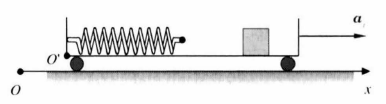
\includegraphics[scale=0.8]{carrello}
    \centering
    \caption{}
    \label{carrello}
\end{figure}

Consideriamo di avere un punto materiale di massa \(m\), posto sul pavimento del carrello che continua a muoversi con accelerazione \(\overrightarrow{a}\). 
Si assuma l'attrito nullo e che ad un estremo del carrello ci sia una molla di costante elastica \(k\) (figura \ref{carrello}).
Nel sistema inerziale si osservano i seguenti eventi: il punto resta fermo (non c'è attrito tra punto e pavimento) mentre il carrello gli scorre sotto, fino a quando l'estremo della molla lo raggiunge. 
La molla inizia allora a comprimersi e il punto a muoversi; a regime il punto è fermo rispetto al carrello mentre è in moto, con la stessa accelerazione \(a\), del carrello, rispetto ad \(O\). 
In tale condizione la molla è compressa dalla quantità \(x_C = m a_t / k\): infatti è la forza elastica della molla, \(k x\), che applicata al punto gli comunica l'accelerazione \(a_t\).

Per l'osservatore \(O'\), posto sul carrello, inizialmente il punto è in moto con accelerazione \(-\overrightarrow{a}_{t}\). 
Infatti \(\overrightarrow{a}' = \overrightarrow{a} -\overrightarrow{a_t}= -\overrightarrow{a_t} \), dato che \(\overrightarrow{a} = 0\). 
Ad un certo istante il punto raggiunge la molla che si comprime e, di conseguenza, il punto si ferma; la molla resta compressa della quantità \(x_c\). 
\(O'\) conclude che sul punto, che sembrerebbe libero, agisce la forza \(-m \overrightarrow{a}\), tanto è vero che quando il punto tocca la molla la comprime. 
Poiché il punto appare da quell'istante fermo, si deduce che in modulo \(k x_c = m a_t\). 
Posso quindi, partendo da \(x_c\) ricavare \(a_t\) (la molla diventa una sorta di accelerometro).

\subsection{Esempio ascensore}

Nell'ultimo esempio ho un asse \(z\) verticale con origine in \(O\) e un secondo asse \(z'\) verticale, con origine in \(O'\), solidale con un ascensore; 
entrambi gli assi sono orientati verso l'alto. 
L'ascensore inizia a salire con accelerazione \(\overrightarrow{a}_t\), descrive successivamente un moto uniforme ed infine decelera con accelerazione \(-\overrightarrow{a}_t\), fino a fermarsi; \(a_t\) è costante in modulo.
L'osservatore nel sistema \(O'\) compie nell'ascensore esperimenti di caduta libera di corpi, misurandone l'accelerazione \(\overrightarrow{a}'\).
Per l'osservatore in \(O\) l'accelerazione dei corpi lasciati cadere da \(O'\) è sempre pari a \(g\). 
In base a (\ref{f_rel}) ho che \(\overrightarrow{g} =\overrightarrow{a}'+ \overrightarrow{a}_t\), e proiettando tale relazione sull'asse \(z\) si ha:
\begin{itemize}
    \item nella fase di accelerazione \(-g = a' + a_t \implies a' = -(g + a_t)\)
    \item nella fase di moto uniforme \(-g = a' \implies a' = -g\)
    \item nella fase di decelerazione \(-g = a' - a_t \implies a' = -(g-a_t)\) 
\end{itemize}
Nella fase di accelerazione \(O'\) constata che i corpi cadono con una accelerazione maggiore di quella di gravità,
nella fase uniforme si torna all'accelerazione normale, mentre nella fase di decelerazione i corpi cadono con una accelerazione minore di \(g\) (diminuzione apparente del peso).

Se fosse \(\overrightarrow{a}_t = \overrightarrow{g}\), come potrebbe accadere nella fase di decelerazione, oppure se l'ascensore scendesse in caduta libera, si troverebbe \(\overrightarrow{a}'= 0\): 
un corpo abbandonato nell'ascensore con velocità iniziale nulla resta fermo rispetto ad \(O'\). \\
È la cosiddetta assenza di peso, avvertita da chi sta dentro l'ascensore e dovuta ovviamente non a una scomparsa reale dell'attrazione terrestre, ma al fatto che se tutto il sistema sta scendendo con la stessa accelerazione dei corpi che ad esso si riferiscono non c'è più accelerazione relativa e, tra l'altro, vengono a mancare le sensazioni ad essa connesse. 
Un effetto analogo, come è ben noto, si manifesta nei satelliti artificiali che ruotano intorno alla terra.

La spiegazione dell'assenza di accelerazione di gravità è quella data da \(O\) che misura in ogni caso \(g\) e ragiona in base a (\ref{f_rel}), attribuendo le variazioni all'accelerazione di trascinamento di \(O'\).
Ma \(O'\), se non ha a priori questo tipo di informazioni, ragiona in modo diverso. 
Egli vede che in certe situazioni l'accelerazione di un corpo che cade è \(g\), in accordo con quanto gli può essere comunicato dall'esterno, ma sperimenta anche situazioni diverse. 
\(O'\) postula pertanto che in certe situazioni, che è capace di mettere in evidenza, ha origine un'accelerazione supplementare che si compone con \(g\) per dare i risultati osservati ovvero che alla forza peso va aggiunto il termine \(-m \overrightarrow{a}_{suppl}\); sulle cause del fenomeno non è però in grado di fare alcuna ipotesi.

Notiamo che dall'esame delle misure di \(a'\) e \(a_{suppl}\) egli sarebbe in grado di accorgersi da solo che c'è un valore speciale, appunto \(g\), che si ottiene sempre sommando o sottraendo i valori di \(a'\) e \(a_{suppl}\); solo in seguito a un'informazione esterna potrebbe però accorgersi che \(a_{suppl}\) non è altro che \(a_t\) e che quindi egli ha un modo per mettere in evidenza cosa sta succedendo al suo sistema.

\end{document}
